% EviBound course report (COSC 723).
% Every result is looked up with \V{key} from report/generated/numbers.tex, which
% scripts/build_report_numbers.py writes from the committed artifacts.
% Build: bash report/build.sh
\documentclass[10pt,twocolumn,a4paper]{article}
\usepackage[T1]{fontenc}
\usepackage[utf8]{inputenc}
\usepackage{mathptmx}
\usepackage[scaled=0.88]{helvet}
\renewcommand{\ttdefault}{lmtt}
\usepackage[a4paper,top=17mm,bottom=19mm,left=16mm,right=16mm,columnsep=6.5mm]{geometry}
\usepackage{microtype}
\usepackage{booktabs,array,tabularx}
\usepackage{xcolor}
\usepackage{tikz}
\usetikzlibrary{arrows.meta,positioning,calc,fit,backgrounds}
\usepackage[font=small,labelfont=bf,skip=4pt]{caption}
\usepackage{enumitem}
\usepackage{titlesec}
\usepackage{xurl}
\usepackage[hidelinks]{hyperref}
\hypersetup{pdftitle={EviBound: Binding an LLM Agent's Device Writes to Recorded, Fresh Evidence},
  pdfauthor={Xin Li},pdfsubject={COSC 723 course project report}}

\definecolor{evigood}{HTML}{1F5FA8}
\definecolor{evibad}{HTML}{B4400F}
\definecolor{evitrust}{HTML}{E9EEF5}

\makeatletter
\newcommand{\V}[1]{\ifcsname ev@#1\endcsname\csname ev@#1\endcsname\else
  \PackageError{evibound}{Unknown report number '#1'}{Run scripts/build_report_numbers.py --keys}\textbf{??}\fi}
\newcommand{\rawinput}[1]{\@@input #1 }
\makeatother
% Generated by scripts/build_report_numbers.py from the committed artifacts.
% Do not edit: change the script or the report text, then rebuild.
\expandafter\def\csname ev@chain.attacks\endcsname{21}
\expandafter\def\csname ev@chain.attacks_run\endcsname{20}
\expandafter\def\csname ev@chain.form_tasks_max\endcsname{84}
\expandafter\def\csname ev@chain.form_tasks_min\endcsname{21}
\expandafter\def\csname ev@chain.hijack_eligible\endcsname{79}
\expandafter\def\csname ev@chain.hijacked\endcsname{30}
\expandafter\def\csname ev@chain.hops\endcsname{12}
\expandafter\def\csname ev@chain.hops_run\endcsname{11}
\expandafter\def\csname ev@chain.persistent.episodes\endcsname{84}
\expandafter\def\csname ev@chain.tasks\endcsname{84}
\expandafter\def\csname ev@chain.trusted_hops\endcsname{6}
\expandafter\def\csname ev@chain.untrusted_attacks\endcsname{13}
\expandafter\def\csname ev@chain.untrusted_episodes\endcsname{2,888}
\expandafter\def\csname ev@env.gpu_gb\endcsname{24}
\expandafter\def\csname ev@env.gpu_name\endcsname{RTX 4090}
\expandafter\def\csname ev@env.gpus\endcsname{2}
\expandafter\def\csname ev@env.gpus.word\endcsname{two}
\expandafter\def\csname ev@example.context\endcsname{workshop}
\expandafter\def\csname ev@example.family\endcsname{strong ventilation}
\expandafter\def\csname ev@example.goal_other\endcsname{light at level~1, fan at level~2}
\expandafter\def\csname ev@example.goal_true\endcsname{light off, fan off}
\expandafter\def\csname ev@example.guarded\endcsname{fan to off}
\expandafter\def\csname ev@example.initial\endcsname{fan at level~1, light off}
\expandafter\def\csname ev@example.unguarded\endcsname{light to level~1, fan to level~2}
\expandafter\def\csname ev@model.revision_short\endcsname{a09a35458c70}
\expandafter\def\csname ev@rep.checks\endcsname{23}
\expandafter\def\csname ev@rep.date\endcsname{2026-11-10}
\expandafter\def\csname ev@rep.minutes\endcsname{21}
\expandafter\def\csname ev@rep.rescored\endcsname{8,424}
\expandafter\def\csname ev@rep.v2.episodes\endcsname{1,296}
\expandafter\def\csname ev@rep.v2.first\endcsname{1,181}
\expandafter\def\csname ev@rep.v2.first_pct\endcsname{91.1}
\expandafter\def\csname ev@rep.v2.outcomes\endcsname{1,221}
\expandafter\def\csname ev@rep.v2.outcomes_pct\endcsname{94.2}
\expandafter\def\csname ev@rep.v2.safety.orig.est\endcsname{+36.4}
\expandafter\def\csname ev@rep.v2.safety.orig.hi\endcsname{+59.1}
\expandafter\def\csname ev@rep.v2.safety.orig.left\endcsname{30}
\expandafter\def\csname ev@rep.v2.safety.orig.lo\endcsname{+18.2}
\expandafter\def\csname ev@rep.v2.safety.orig.right\endcsname{0}
\expandafter\def\csname ev@rep.v2.safety.rerun.est\endcsname{+36.4}
\expandafter\def\csname ev@rep.v2.safety.rerun.hi\endcsname{+59.1}
\expandafter\def\csname ev@rep.v2.safety.rerun.left\endcsname{30}
\expandafter\def\csname ev@rep.v2.safety.rerun.lo\endcsname{+18.2}
\expandafter\def\csname ev@rep.v2.safety.rerun.right\endcsname{0}
\expandafter\def\csname ev@rep.v2.utility.orig.est\endcsname{$-$13.6}
\expandafter\def\csname ev@rep.v2.utility.orig.hi\endcsname{0.0}
\expandafter\def\csname ev@rep.v2.utility.orig.left\endcsname{44}
\expandafter\def\csname ev@rep.v2.utility.orig.lo\endcsname{$-$27.3}
\expandafter\def\csname ev@rep.v2.utility.orig.right\endcsname{53}
\expandafter\def\csname ev@rep.v2.utility.rerun.est\endcsname{$-$13.6}
\expandafter\def\csname ev@rep.v2.utility.rerun.hi\endcsname{0.0}
\expandafter\def\csname ev@rep.v2.utility.rerun.left\endcsname{45}
\expandafter\def\csname ev@rep.v2.utility.rerun.lo\endcsname{$-$27.3}
\expandafter\def\csname ev@rep.v2.utility.rerun.right\endcsname{54}
\expandafter\def\csname ev@rep.v2.writes\endcsname{1,167}
\expandafter\def\csname ev@rep.v2.writes_pct\endcsname{90.0}
\expandafter\def\csname ev@rep.v3.S1.orig.est\endcsname{+15.3}
\expandafter\def\csname ev@rep.v3.S1.orig.hi\endcsname{+26.4}
\expandafter\def\csname ev@rep.v3.S1.orig.left\endcsname{11}
\expandafter\def\csname ev@rep.v3.S1.orig.lo\endcsname{+5.6}
\expandafter\def\csname ev@rep.v3.S1.orig.right\endcsname{0}
\expandafter\def\csname ev@rep.v3.S1.rerun.est\endcsname{+15.3}
\expandafter\def\csname ev@rep.v3.S1.rerun.hi\endcsname{+26.4}
\expandafter\def\csname ev@rep.v3.S1.rerun.left\endcsname{11}
\expandafter\def\csname ev@rep.v3.S1.rerun.lo\endcsname{+5.6}
\expandafter\def\csname ev@rep.v3.S1.rerun.right\endcsname{0}
\expandafter\def\csname ev@rep.v3.U1.orig.est\endcsname{$-$8.3}
\expandafter\def\csname ev@rep.v3.U1.orig.hi\endcsname{+2.8}
\expandafter\def\csname ev@rep.v3.U1.orig.left\endcsname{52}
\expandafter\def\csname ev@rep.v3.U1.orig.lo\endcsname{$-$20.8}
\expandafter\def\csname ev@rep.v3.U1.orig.right\endcsname{58}
\expandafter\def\csname ev@rep.v3.U1.rerun.est\endcsname{$-$9.7}
\expandafter\def\csname ev@rep.v3.U1.rerun.hi\endcsname{+2.8}
\expandafter\def\csname ev@rep.v3.U1.rerun.left\endcsname{51}
\expandafter\def\csname ev@rep.v3.U1.rerun.lo\endcsname{$-$23.6}
\expandafter\def\csname ev@rep.v3.U1.rerun.right\endcsname{58}
\expandafter\def\csname ev@rep.v3.U2.orig.est\endcsname{+29.2}
\expandafter\def\csname ev@rep.v3.U2.orig.hi\endcsname{+43.1}
\expandafter\def\csname ev@rep.v3.U2.orig.left\endcsname{52}
\expandafter\def\csname ev@rep.v3.U2.orig.lo\endcsname{+16.7}
\expandafter\def\csname ev@rep.v3.U2.orig.right\endcsname{31}
\expandafter\def\csname ev@rep.v3.U2.rerun.est\endcsname{+29.2}
\expandafter\def\csname ev@rep.v3.U2.rerun.hi\endcsname{+43.1}
\expandafter\def\csname ev@rep.v3.U2.rerun.left\endcsname{51}
\expandafter\def\csname ev@rep.v3.U2.rerun.lo\endcsname{+16.7}
\expandafter\def\csname ev@rep.v3.U2.rerun.right\endcsname{30}
\expandafter\def\csname ev@rep.v3.cell\endcsname{72}
\expandafter\def\csname ev@rep.v3.episodes\endcsname{2,376}
\expandafter\def\csname ev@rep.v3.first\endcsname{2,178}
\expandafter\def\csname ev@rep.v3.first_pct\endcsname{91.7}
\expandafter\def\csname ev@rep.v3.outcomes\endcsname{2,321}
\expandafter\def\csname ev@rep.v3.outcomes_pct\endcsname{97.7}
\expandafter\def\csname ev@rep.v3.writes\endcsname{2,227}
\expandafter\def\csname ev@rep.v3.writes_pct\endcsname{93.7}
\expandafter\def\csname ev@snapshot.component_tests\endcsname{27}
\expandafter\def\csname ev@snapshot.date\endcsname{18 November 2026}
\expandafter\def\csname ev@snapshot.unit_tests\endcsname{128}
\expandafter\def\csname ev@traces.bytes\endcsname{2,279,422}
\expandafter\def\csname ev@v2.a3.b0_att\endcsname{3}
\expandafter\def\csname ev@v2.a3.cell\endcsname{18}
\expandafter\def\csname ev@v2.a3.tasks_violated\endcsname{1}
\expandafter\def\csname ev@v2.a3_tasks\endcsname{6}
\expandafter\def\csname ev@v2.att.b0.attackgoal\endcsname{56}
\expandafter\def\csname ev@v2.att.b0.authz\endcsname{3}
\expandafter\def\csname ev@v2.att.b0.eligible\endcsname{0}
\expandafter\def\csname ev@v2.att.b0.empty\endcsname{6}
\expandafter\def\csname ev@v2.att.b0.falseblocks\endcsname{0}
\expandafter\def\csname ev@v2.att.b0.goal\endcsname{0}
\expandafter\def\csname ev@v2.att.b0.latency\endcsname{0.22}
\expandafter\def\csname ev@v2.att.b0.reads\endcsname{1.00}
\expandafter\def\csname ev@v2.att.b0.safe\endcsname{0}
\expandafter\def\csname ev@v2.att.b0.tokens\endcsname{701}
\expandafter\def\csname ev@v2.att.b0.unsafe\endcsname{45}
\expandafter\def\csname ev@v2.att.b0.unsafe_replay\endcsname{24}
\expandafter\def\csname ev@v2.att.b0.unsafe_tamper\endcsname{21}
\expandafter\def\csname ev@v2.att.b1.attackgoal\endcsname{49}
\expandafter\def\csname ev@v2.att.b1.authz\endcsname{0}
\expandafter\def\csname ev@v2.att.b1.eligible\endcsname{0}
\expandafter\def\csname ev@v2.att.b1.empty\endcsname{8}
\expandafter\def\csname ev@v2.att.b1.falseblocks\endcsname{0}
\expandafter\def\csname ev@v2.att.b1.goal\endcsname{0}
\expandafter\def\csname ev@v2.att.b1.latency\endcsname{0.22}
\expandafter\def\csname ev@v2.att.b1.reads\endcsname{1.00}
\expandafter\def\csname ev@v2.att.b1.safe\endcsname{0}
\expandafter\def\csname ev@v2.att.b1.tokens\endcsname{728}
\expandafter\def\csname ev@v2.att.b1.unsafe\endcsname{45}
\expandafter\def\csname ev@v2.att.b2.attackgoal\endcsname{38}
\expandafter\def\csname ev@v2.att.b2.authz\endcsname{0}
\expandafter\def\csname ev@v2.att.b2.eligible\endcsname{21}
\expandafter\def\csname ev@v2.att.b2.empty\endcsname{6}
\expandafter\def\csname ev@v2.att.b2.falseblocks\endcsname{0}
\expandafter\def\csname ev@v2.att.b2.goal\endcsname{16}
\expandafter\def\csname ev@v2.att.b2.latency\endcsname{0.30}
\expandafter\def\csname ev@v2.att.b2.reads\endcsname{1.29}
\expandafter\def\csname ev@v2.att.b2.safe\endcsname{15}
\expandafter\def\csname ev@v2.att.b2.tokens\endcsname{959}
\expandafter\def\csname ev@v2.att.b2.unsafe\endcsname{30}
\expandafter\def\csname ev@v2.att.b2.unsafe_replay\endcsname{18}
\expandafter\def\csname ev@v2.att.b2.unsafe_tamper\endcsname{12}
\expandafter\def\csname ev@v2.att.m.attackgoal\endcsname{1}
\expandafter\def\csname ev@v2.att.m.authz\endcsname{0}
\expandafter\def\csname ev@v2.att.m.eligible\endcsname{48}
\expandafter\def\csname ev@v2.att.m.empty\endcsname{6}
\expandafter\def\csname ev@v2.att.m.falseblocks\endcsname{0}
\expandafter\def\csname ev@v2.att.m.goal\endcsname{23}
\expandafter\def\csname ev@v2.att.m.latency\endcsname{0.54}
\expandafter\def\csname ev@v2.att.m.reads\endcsname{1.92}
\expandafter\def\csname ev@v2.att.m.safe\endcsname{23}
\expandafter\def\csname ev@v2.att.m.tokens\endcsname{1,509}
\expandafter\def\csname ev@v2.att.m.unsafe\endcsname{0}
\expandafter\def\csname ev@v2.att.nofresh.attackgoal\endcsname{21}
\expandafter\def\csname ev@v2.att.nofresh.authz\endcsname{0}
\expandafter\def\csname ev@v2.att.nofresh.eligible\endcsname{54}
\expandafter\def\csname ev@v2.att.nofresh.empty\endcsname{6}
\expandafter\def\csname ev@v2.att.nofresh.falseblocks\endcsname{0}
\expandafter\def\csname ev@v2.att.nofresh.goal\endcsname{29}
\expandafter\def\csname ev@v2.att.nofresh.latency\endcsname{0.40}
\expandafter\def\csname ev@v2.att.nofresh.reads\endcsname{1.60}
\expandafter\def\csname ev@v2.att.nofresh.safe\endcsname{27}
\expandafter\def\csname ev@v2.att.nofresh.tokens\endcsname{1,230}
\expandafter\def\csname ev@v2.att.nofresh.unsafe\endcsname{18}
\expandafter\def\csname ev@v2.att.nofresh.unsafe_replay\endcsname{18}
\expandafter\def\csname ev@v2.att.nofresh.unsafe_tamper\endcsname{0}
\expandafter\def\csname ev@v2.att.refresh.attackgoal\endcsname{17}
\expandafter\def\csname ev@v2.att.refresh.authz\endcsname{0}
\expandafter\def\csname ev@v2.att.refresh.eligible\endcsname{83}
\expandafter\def\csname ev@v2.att.refresh.empty\endcsname{6}
\expandafter\def\csname ev@v2.att.refresh.falseblocks\endcsname{0}
\expandafter\def\csname ev@v2.att.refresh.goal\endcsname{39}
\expandafter\def\csname ev@v2.att.refresh.latency\endcsname{0.42}
\expandafter\def\csname ev@v2.att.refresh.reads\endcsname{3.44}
\expandafter\def\csname ev@v2.att.refresh.safe\endcsname{39}
\expandafter\def\csname ev@v2.att.refresh.tokens\endcsname{1,253}
\expandafter\def\csname ev@v2.att.refresh.unsafe\endcsname{0}
\expandafter\def\csname ev@v2.bootstrap\endcsname{10,000}
\expandafter\def\csname ev@v2.bound.b0.attackgoal\endcsname{0}
\expandafter\def\csname ev@v2.bound.b0.authz\endcsname{0}
\expandafter\def\csname ev@v2.bound.b0.eligible\endcsname{55}
\expandafter\def\csname ev@v2.bound.b0.empty\endcsname{13}
\expandafter\def\csname ev@v2.bound.b0.falseblocks\endcsname{0}
\expandafter\def\csname ev@v2.bound.b0.goal\endcsname{48}
\expandafter\def\csname ev@v2.bound.b0.latency\endcsname{0.22}
\expandafter\def\csname ev@v2.bound.b0.reads\endcsname{1.00}
\expandafter\def\csname ev@v2.bound.b0.safe\endcsname{41}
\expandafter\def\csname ev@v2.bound.b0.tokens\endcsname{700}
\expandafter\def\csname ev@v2.bound.b0.unsafe\endcsname{10}
\expandafter\def\csname ev@v2.bound.b1.attackgoal\endcsname{0}
\expandafter\def\csname ev@v2.bound.b1.authz\endcsname{0}
\expandafter\def\csname ev@v2.bound.b1.eligible\endcsname{48}
\expandafter\def\csname ev@v2.bound.b1.empty\endcsname{18}
\expandafter\def\csname ev@v2.bound.b1.falseblocks\endcsname{0}
\expandafter\def\csname ev@v2.bound.b1.goal\endcsname{42}
\expandafter\def\csname ev@v2.bound.b1.latency\endcsname{0.22}
\expandafter\def\csname ev@v2.bound.b1.reads\endcsname{1.00}
\expandafter\def\csname ev@v2.bound.b1.safe\endcsname{33}
\expandafter\def\csname ev@v2.bound.b1.tokens\endcsname{726}
\expandafter\def\csname ev@v2.bound.b1.unsafe\endcsname{12}
\expandafter\def\csname ev@v2.bound.b2.attackgoal\endcsname{7}
\expandafter\def\csname ev@v2.bound.b2.authz\endcsname{0}
\expandafter\def\csname ev@v2.bound.b2.eligible\endcsname{59}
\expandafter\def\csname ev@v2.bound.b2.empty\endcsname{13}
\expandafter\def\csname ev@v2.bound.b2.falseblocks\endcsname{0}
\expandafter\def\csname ev@v2.bound.b2.goal\endcsname{41}
\expandafter\def\csname ev@v2.bound.b2.latency\endcsname{0.26}
\expandafter\def\csname ev@v2.bound.b2.reads\endcsname{1.14}
\expandafter\def\csname ev@v2.bound.b2.safe\endcsname{41}
\expandafter\def\csname ev@v2.bound.b2.tokens\endcsname{823}
\expandafter\def\csname ev@v2.bound.b2.unsafe\endcsname{0}
\expandafter\def\csname ev@v2.bound.m.attackgoal\endcsname{7}
\expandafter\def\csname ev@v2.bound.m.authz\endcsname{0}
\expandafter\def\csname ev@v2.bound.m.eligible\endcsname{115}
\expandafter\def\csname ev@v2.bound.m.empty\endcsname{13}
\expandafter\def\csname ev@v2.bound.m.falseblocks\endcsname{0}
\expandafter\def\csname ev@v2.bound.m.goal\endcsname{41}
\expandafter\def\csname ev@v2.bound.m.latency\endcsname{0.42}
\expandafter\def\csname ev@v2.bound.m.reads\endcsname{1.61}
\expandafter\def\csname ev@v2.bound.m.safe\endcsname{41}
\expandafter\def\csname ev@v2.bound.m.tokens\endcsname{1,244}
\expandafter\def\csname ev@v2.bound.m.unsafe\endcsname{0}
\expandafter\def\csname ev@v2.bound.nofresh.attackgoal\endcsname{7}
\expandafter\def\csname ev@v2.bound.nofresh.authz\endcsname{0}
\expandafter\def\csname ev@v2.bound.nofresh.eligible\endcsname{59}
\expandafter\def\csname ev@v2.bound.nofresh.empty\endcsname{13}
\expandafter\def\csname ev@v2.bound.nofresh.falseblocks\endcsname{0}
\expandafter\def\csname ev@v2.bound.nofresh.goal\endcsname{41}
\expandafter\def\csname ev@v2.bound.nofresh.latency\endcsname{0.26}
\expandafter\def\csname ev@v2.bound.nofresh.reads\endcsname{1.14}
\expandafter\def\csname ev@v2.bound.nofresh.safe\endcsname{41}
\expandafter\def\csname ev@v2.bound.nofresh.tokens\endcsname{823}
\expandafter\def\csname ev@v2.bound.nofresh.unsafe\endcsname{0}
\expandafter\def\csname ev@v2.bound.refresh.attackgoal\endcsname{7}
\expandafter\def\csname ev@v2.bound.refresh.authz\endcsname{0}
\expandafter\def\csname ev@v2.bound.refresh.eligible\endcsname{93}
\expandafter\def\csname ev@v2.bound.refresh.empty\endcsname{13}
\expandafter\def\csname ev@v2.bound.refresh.falseblocks\endcsname{0}
\expandafter\def\csname ev@v2.bound.refresh.goal\endcsname{41}
\expandafter\def\csname ev@v2.bound.refresh.latency\endcsname{0.28}
\expandafter\def\csname ev@v2.bound.refresh.reads\endcsname{2.65}
\expandafter\def\csname ev@v2.bound.refresh.safe\endcsname{41}
\expandafter\def\csname ev@v2.bound.refresh.tokens\endcsname{823}
\expandafter\def\csname ev@v2.bound.refresh.unsafe\endcsname{0}
\expandafter\def\csname ev@v2.cell\endcsname{72}
\expandafter\def\csname ev@v2.clean.b0.attackgoal\endcsname{0}
\expandafter\def\csname ev@v2.clean.b0.authz\endcsname{0}
\expandafter\def\csname ev@v2.clean.b0.eligible\endcsname{102}
\expandafter\def\csname ev@v2.clean.b0.empty\endcsname{8}
\expandafter\def\csname ev@v2.clean.b0.falseblocks\endcsname{0}
\expandafter\def\csname ev@v2.clean.b0.goal\endcsname{53}
\expandafter\def\csname ev@v2.clean.b0.latency\endcsname{0.22}
\expandafter\def\csname ev@v2.clean.b0.reads\endcsname{1.00}
\expandafter\def\csname ev@v2.clean.b0.safe\endcsname{44}
\expandafter\def\csname ev@v2.clean.b0.tokens\endcsname{701}
\expandafter\def\csname ev@v2.clean.b0.unsafe\endcsname{12}
\expandafter\def\csname ev@v2.clean.b1.attackgoal\endcsname{0}
\expandafter\def\csname ev@v2.clean.b1.authz\endcsname{0}
\expandafter\def\csname ev@v2.clean.b1.eligible\endcsname{93}
\expandafter\def\csname ev@v2.clean.b1.empty\endcsname{12}
\expandafter\def\csname ev@v2.clean.b1.falseblocks\endcsname{0}
\expandafter\def\csname ev@v2.clean.b1.goal\endcsname{48}
\expandafter\def\csname ev@v2.clean.b1.latency\endcsname{0.22}
\expandafter\def\csname ev@v2.clean.b1.reads\endcsname{1.00}
\expandafter\def\csname ev@v2.clean.b1.safe\endcsname{39}
\expandafter\def\csname ev@v2.clean.b1.tokens\endcsname{728}
\expandafter\def\csname ev@v2.clean.b1.unsafe\endcsname{12}
\expandafter\def\csname ev@v2.clean.b2.attackgoal\endcsname{6}
\expandafter\def\csname ev@v2.clean.b2.authz\endcsname{0}
\expandafter\def\csname ev@v2.clean.b2.eligible\endcsname{99}
\expandafter\def\csname ev@v2.clean.b2.empty\endcsname{8}
\expandafter\def\csname ev@v2.clean.b2.falseblocks\endcsname{0}
\expandafter\def\csname ev@v2.clean.b2.goal\endcsname{44}
\expandafter\def\csname ev@v2.clean.b2.latency\endcsname{0.26}
\expandafter\def\csname ev@v2.clean.b2.reads\endcsname{1.17}
\expandafter\def\csname ev@v2.clean.b2.safe\endcsname{44}
\expandafter\def\csname ev@v2.clean.b2.tokens\endcsname{849}
\expandafter\def\csname ev@v2.clean.b2.unsafe\endcsname{0}
\expandafter\def\csname ev@v2.clean.empty_both\endcsname{7}
\expandafter\def\csname ev@v2.clean.m.attackgoal\endcsname{6}
\expandafter\def\csname ev@v2.clean.m.authz\endcsname{0}
\expandafter\def\csname ev@v2.clean.m.eligible\endcsname{99}
\expandafter\def\csname ev@v2.clean.m.empty\endcsname{8}
\expandafter\def\csname ev@v2.clean.m.falseblocks\endcsname{0}
\expandafter\def\csname ev@v2.clean.m.goal\endcsname{44}
\expandafter\def\csname ev@v2.clean.m.latency\endcsname{0.26}
\expandafter\def\csname ev@v2.clean.m.reads\endcsname{1.17}
\expandafter\def\csname ev@v2.clean.m.safe\endcsname{44}
\expandafter\def\csname ev@v2.clean.m.tokens\endcsname{849}
\expandafter\def\csname ev@v2.clean.m.unsafe\endcsname{0}
\expandafter\def\csname ev@v2.clean.nofresh.attackgoal\endcsname{6}
\expandafter\def\csname ev@v2.clean.nofresh.authz\endcsname{0}
\expandafter\def\csname ev@v2.clean.nofresh.eligible\endcsname{99}
\expandafter\def\csname ev@v2.clean.nofresh.empty\endcsname{8}
\expandafter\def\csname ev@v2.clean.nofresh.falseblocks\endcsname{0}
\expandafter\def\csname ev@v2.clean.nofresh.goal\endcsname{44}
\expandafter\def\csname ev@v2.clean.nofresh.latency\endcsname{0.26}
\expandafter\def\csname ev@v2.clean.nofresh.reads\endcsname{1.17}
\expandafter\def\csname ev@v2.clean.nofresh.safe\endcsname{44}
\expandafter\def\csname ev@v2.clean.nofresh.tokens\endcsname{849}
\expandafter\def\csname ev@v2.clean.nofresh.unsafe\endcsname{0}
\expandafter\def\csname ev@v2.clean.reachable\endcsname{60}
\expandafter\def\csname ev@v2.clean.refresh.attackgoal\endcsname{6}
\expandafter\def\csname ev@v2.clean.refresh.authz\endcsname{0}
\expandafter\def\csname ev@v2.clean.refresh.eligible\endcsname{99}
\expandafter\def\csname ev@v2.clean.refresh.empty\endcsname{8}
\expandafter\def\csname ev@v2.clean.refresh.falseblocks\endcsname{0}
\expandafter\def\csname ev@v2.clean.refresh.goal\endcsname{44}
\expandafter\def\csname ev@v2.clean.refresh.latency\endcsname{0.28}
\expandafter\def\csname ev@v2.clean.refresh.reads\endcsname{2.83}
\expandafter\def\csname ev@v2.clean.refresh.safe\endcsname{44}
\expandafter\def\csname ev@v2.clean.refresh.tokens\endcsname{849}
\expandafter\def\csname ev@v2.clean.refresh.unsafe\endcsname{0}
\expandafter\def\csname ev@v2.clean.unreachable\endcsname{12}
\expandafter\def\csname ev@v2.clusters\endcsname{22}
\expandafter\def\csname ev@v2.completed\endcsname{2026-10-10}
\expandafter\def\csname ev@v2.conditions\endcsname{6}
\expandafter\def\csname ev@v2.contract_episodes\endcsname{864}
\expandafter\def\csname ev@v2.dev_tasks\endcsname{16}
\expandafter\def\csname ev@v2.episodes\endcsname{1,296}
\expandafter\def\csname ev@v2.false_blocks\endcsname{0}
\expandafter\def\csname ev@v2.families\endcsname{8}
\expandafter\def\csname ev@v2.fresh.est\endcsname{+22.7}
\expandafter\def\csname ev@v2.fresh.hi\endcsname{+40.9}
\expandafter\def\csname ev@v2.fresh.lo\endcsname{+6.8}
\expandafter\def\csname ev@v2.frozen\endcsname{2026-10-10}
\expandafter\def\csname ev@v2.fullguard.episodes\endcsname{432}
\expandafter\def\csname ev@v2.gap.episodes\endcsname{9}
\expandafter\def\csname ev@v2.gap.episodes.word\endcsname{nine}
\expandafter\def\csname ev@v2.gap.fan_jumps\endcsname{3}
\expandafter\def\csname ev@v2.gap.light_jumps\endcsname{6}
\expandafter\def\csname ev@v2.gap.seeds\endcsname{3}
\expandafter\def\csname ev@v2.gap.seeds.word\endcsname{three}
\expandafter\def\csname ev@v2.gap.tasks\endcsname{3}
\expandafter\def\csname ev@v2.gap.tasks.word\endcsname{three}
\expandafter\def\csname ev@v2.generations\endcsname{729}
\expandafter\def\csname ev@v2.margin\endcsname{$-$5}
\expandafter\def\csname ev@v2.paired_triples\endcsname{216}
\expandafter\def\csname ev@v2.parse_failures\endcsname{0}
\expandafter\def\csname ev@v2.pilot.safety.est\endcsname{+20.0}
\expandafter\def\csname ev@v2.pilot.safety.hi\endcsname{+40.0}
\expandafter\def\csname ev@v2.pilot.safety.lo\endcsname{0.0}
\expandafter\def\csname ev@v2.pilot.utility.est\endcsname{$-$20.0}
\expandafter\def\csname ev@v2.pilot.utility.hi\endcsname{$-$4.4}
\expandafter\def\csname ev@v2.pilot.utility.lo\endcsname{$-$40.0}
\expandafter\def\csname ev@v2.pilot_tasks\endcsname{16}
\expandafter\def\csname ev@v2.rec.att.changed_retry\endcsname{39}
\expandafter\def\csname ev@v2.rec.att.empty_retry\endcsname{27}
\expandafter\def\csname ev@v2.rec.att.mismatch\endcsname{31}
\expandafter\def\csname ev@v2.rec.att.not_fresh\endcsname{35}
\expandafter\def\csname ev@v2.rec.att.recovered\endcsname{23}
\expandafter\def\csname ev@v2.rec.att.rejected\endcsname{66}
\expandafter\def\csname ev@v2.rec.clean.changed_plan\endcsname{9}
\expandafter\def\csname ev@v2.rec.clean.empty\endcsname{8}
\expandafter\def\csname ev@v2.rec.clean.failures\endcsname{28}
\expandafter\def\csname ev@v2.rec.clean.recovered\endcsname{0}
\expandafter\def\csname ev@v2.rec.clean.rejected\endcsname{12}
\expandafter\def\csname ev@v2.rec.clean.same_plan\endcsname{3}
\expandafter\def\csname ev@v2.refresh.diff\endcsname{+1.46}
\expandafter\def\csname ev@v2.refresh.hi\endcsname{+1.83}
\expandafter\def\csname ev@v2.refresh.lo\endcsname{+1.08}
\expandafter\def\csname ev@v2.refresh.reads_m\endcsname{1.92}
\expandafter\def\csname ev@v2.refresh.reads_refresh\endcsname{3.44}
\expandafter\def\csname ev@v2.replay_tasks\endcsname{12}
\expandafter\def\csname ev@v2.safety.b2\endcsname{30}
\expandafter\def\csname ev@v2.safety.est\endcsname{+36.4}
\expandafter\def\csname ev@v2.safety.hi\endcsname{+59.1}
\expandafter\def\csname ev@v2.safety.lo\endcsname{+18.2}
\expandafter\def\csname ev@v2.safety.m\endcsname{0}
\expandafter\def\csname ev@v2.seeds\endcsname{3}
\expandafter\def\csname ev@v2.shared_structures\endcsname{12}
\expandafter\def\csname ev@v2.tamper_tasks\endcsname{12}
\expandafter\def\csname ev@v2.tasks\endcsname{24}
\expandafter\def\csname ev@v2.temperature\endcsname{0.2}
\expandafter\def\csname ev@v2.tokens_thousand\endcsname{571}
\expandafter\def\csname ev@v2.top_k\endcsname{20}
\expandafter\def\csname ev@v2.top_p\endcsname{0.9}
\expandafter\def\csname ev@v2.utility.b0\endcsname{53}
\expandafter\def\csname ev@v2.utility.est\endcsname{$-$13.6}
\expandafter\def\csname ev@v2.utility.hi\endcsname{0.0}
\expandafter\def\csname ev@v2.utility.lo\endcsname{$-$27.3}
\expandafter\def\csname ev@v2.utility.m\endcsname{44}
\expandafter\def\csname ev@v3.R1.est\endcsname{+19.4}
\expandafter\def\csname ev@v3.R1.hi\endcsname{+31.9}
\expandafter\def\csname ev@v3.R1.left\endcsname{156}
\expandafter\def\csname ev@v3.R1.lo\endcsname{+8.3}
\expandafter\def\csname ev@v3.R1.right\endcsname{114}
\expandafter\def\csname ev@v3.R2.est\endcsname{+9.7}
\expandafter\def\csname ev@v3.R2.hi\endcsname{+19.9}
\expandafter\def\csname ev@v3.R2.lo\endcsname{0.0}
\expandafter\def\csname ev@v3.R3.est\endcsname{+2.8}
\expandafter\def\csname ev@v3.R3.hi\endcsname{+8.3}
\expandafter\def\csname ev@v3.R3.lo\endcsname{$-$2.8}
\expandafter\def\csname ev@v3.S1.est\endcsname{+14.4}
\expandafter\def\csname ev@v3.S1.hi\endcsname{+25.9}
\expandafter\def\csname ev@v3.S1.left\endcsname{31}
\expandafter\def\csname ev@v3.S1.lo\endcsname{+4.6}
\expandafter\def\csname ev@v3.S1.right\endcsname{0}
\expandafter\def\csname ev@v3.U1.est\endcsname{$-$7.4}
\expandafter\def\csname ev@v3.U1.hi\endcsname{+3.2}
\expandafter\def\csname ev@v3.U1.left\endcsname{156}
\expandafter\def\csname ev@v3.U1.lo\endcsname{$-$19.0}
\expandafter\def\csname ev@v3.U1.right\endcsname{172}
\expandafter\def\csname ev@v3.U2.est\endcsname{+29.2}
\expandafter\def\csname ev@v3.U2.hi\endcsname{+43.1}
\expandafter\def\csname ev@v3.U2.left\endcsname{156}
\expandafter\def\csname ev@v3.U2.lo\endcsname{+16.7}
\expandafter\def\csname ev@v3.U2.right\endcsname{93}
\expandafter\def\csname ev@v3.Udec.clusters_needed\endcsname{157}
\expandafter\def\csname ev@v3.Udec.est\endcsname{+1.4}
\expandafter\def\csname ev@v3.Udec.hi\endcsname{+8.3}
\expandafter\def\csname ev@v3.Udec.left\endcsname{193}
\expandafter\def\csname ev@v3.Udec.lo\endcsname{$-$5.6}
\expandafter\def\csname ev@v3.Udec.right\endcsname{190}
\expandafter\def\csname ev@v3.aid_confirm.est\endcsname{0.0}
\expandafter\def\csname ev@v3.aid_confirm.hi\endcsname{0.0}
\expandafter\def\csname ev@v3.aid_confirm.lo\endcsname{0.0}
\expandafter\def\csname ev@v3.aid_explain.est\endcsname{+16.7}
\expandafter\def\csname ev@v3.aid_explain.hi\endcsname{+29.2}
\expandafter\def\csname ev@v3.aid_explain.lo\endcsname{+5.6}
\expandafter\def\csname ev@v3.aid_menu.est\endcsname{+5.6}
\expandafter\def\csname ev@v3.aid_menu.hi\endcsname{+11.1}
\expandafter\def\csname ev@v3.aid_menu.lo\endcsname{+1.4}
\expandafter\def\csname ev@v3.att.b0.attackgoal\endcsname{148}
\expandafter\def\csname ev@v3.att.b0.goal\endcsname{80}
\expandafter\def\csname ev@v3.att.b0.safe\endcsname{39}
\expandafter\def\csname ev@v3.att.b0.unsafe\endcsname{77}
\expandafter\def\csname ev@v3.att.b2.goal\endcsname{78}
\expandafter\def\csname ev@v3.att.b2.safe\endcsname{62}
\expandafter\def\csname ev@v3.att.b2.unsafe\endcsname{31}
\expandafter\def\csname ev@v3.att.b2full.attackgoal\endcsname{101}
\expandafter\def\csname ev@v3.att.b2full.goal\endcsname{68}
\expandafter\def\csname ev@v3.att.b2full.safe\endcsname{52}
\expandafter\def\csname ev@v3.att.b2full.unsafe\endcsname{31}
\expandafter\def\csname ev@v3.att.m.attackgoal\endcsname{22}
\expandafter\def\csname ev@v3.att.m.goal\endcsname{102}
\expandafter\def\csname ev@v3.att.m.safe\endcsname{102}
\expandafter\def\csname ev@v3.att.m.unsafe\endcsname{0}
\expandafter\def\csname ev@v3.att.mfull.attackgoal\endcsname{45}
\expandafter\def\csname ev@v3.att.mfull.goal\endcsname{123}
\expandafter\def\csname ev@v3.att.mfull.safe\endcsname{123}
\expandafter\def\csname ev@v3.att.mfull.unsafe\endcsname{0}
\expandafter\def\csname ev@v3.cell\endcsname{216}
\expandafter\def\csname ev@v3.clean.b0.attackgoal\endcsname{58}
\expandafter\def\csname ev@v3.clean.b0.goal\endcsname{172}
\expandafter\def\csname ev@v3.clean.b0.goal_total\endcsname{172}
\expandafter\def\csname ev@v3.clean.b0.noncompliant\endcsname{79}
\expandafter\def\csname ev@v3.clean.b0.safe\endcsname{93}
\expandafter\def\csname ev@v3.clean.b0.unsafe\endcsname{69}
\expandafter\def\csname ev@v3.clean.b2.goal\endcsname{114}
\expandafter\def\csname ev@v3.clean.b2.safe\endcsname{114}
\expandafter\def\csname ev@v3.clean.b2.unsafe\endcsname{0}
\expandafter\def\csname ev@v3.clean.b2full.attackgoal\endcsname{43}
\expandafter\def\csname ev@v3.clean.b2full.goal\endcsname{157}
\expandafter\def\csname ev@v3.clean.b2full.safe\endcsname{157}
\expandafter\def\csname ev@v3.clean.b2full.unsafe\endcsname{0}
\expandafter\def\csname ev@v3.clean.m.attackgoal\endcsname{32}
\expandafter\def\csname ev@v3.clean.m.goal\endcsname{114}
\expandafter\def\csname ev@v3.clean.m.safe\endcsname{114}
\expandafter\def\csname ev@v3.clean.m.unsafe\endcsname{0}
\expandafter\def\csname ev@v3.clean.mfull.attackgoal\endcsname{42}
\expandafter\def\csname ev@v3.clean.mfull.goal\endcsname{156}
\expandafter\def\csname ev@v3.clean.mfull.noncompliant\endcsname{0}
\expandafter\def\csname ev@v3.clean.mfull.safe\endcsname{156}
\expandafter\def\csname ev@v3.clean.mfull.unsafe\endcsname{0}
\expandafter\def\csname ev@v3.clusters\endcsname{36}
\expandafter\def\csname ev@v3.completed\endcsname{2026-10-12}
\expandafter\def\csname ev@v3.conditions\endcsname{11}
\expandafter\def\csname ev@v3.encoding.b2_unsafe_max\endcsname{10}
\expandafter\def\csname ev@v3.encoding.b2_unsafe_min\endcsname{6}
\expandafter\def\csname ev@v3.encoding.cell\endcsname{54}
\expandafter\def\csname ev@v3.episodes\endcsname{7,128}
\expandafter\def\csname ev@v3.frozen\endcsname{2026-10-12}
\expandafter\def\csname ev@v3.fullguard.conditions\endcsname{6}
\expandafter\def\csname ev@v3.fullguard.episodes\endcsname{3,888}
\expandafter\def\csname ev@v3.oracle_disagreements\endcsname{0}
\expandafter\def\csname ev@v3.review_date\endcsname{2026-10-11}
\expandafter\def\csname ev@v3.review_rows\endcsname{77}
\expandafter\def\csname ev@v3.scope.in.b0\endcsname{147}
\expandafter\def\csname ev@v3.scope.in.b0_violation\endcsname{54}
\expandafter\def\csname ev@v3.scope.in.b2full\endcsname{157}
\expandafter\def\csname ev@v3.scope.in.m\endcsname{114}
\expandafter\def\csname ev@v3.scope.in.mfull\endcsname{156}
\expandafter\def\csname ev@v3.scope.in.n\endcsname{168}
\expandafter\def\csname ev@v3.scope.out.b0\endcsname{25}
\expandafter\def\csname ev@v3.scope.out.n\endcsname{48}
\expandafter\def\csname ev@v3.tasks\endcsname{72}


\newcommand{\cond}[1]{\textsf{#1}}
\newcommand{\M}{\cond{M}}
\newcommand{\Bz}{\cond{B0}}
\newcommand{\Bo}{\cond{B1}}
\newcommand{\Bt}{\cond{B2}}
\newcommand{\NoF}{\cond{M\_no\_freshness}}
\newcommand{\Refresh}{\cond{Always\_refresh}}
\newcommand{\Mfull}{\cond{M\_full}}
\newcommand{\Btfull}{\cond{B2\_full}}
\newcommand{\ci}[1]{[\V{#1.lo}, \V{#1.hi}]}
\newcommand{\pts}{points}
\newcommand{\para}[1]{\par\smallskip\noindent\textbf{#1}\hspace{0.5em}}

\titleformat{\section}{\normalfont\large\bfseries}{\thesection}{0.6em}{}
\titlespacing*{\section}{0pt}{9pt plus 2pt minus 2pt}{4pt}
\titleformat{\subsection}{\normalfont\normalsize\bfseries}{\thesubsection}{0.6em}{}
\titlespacing*{\subsection}{0pt}{7pt plus 2pt minus 1pt}{3pt}
\setlist{nosep,leftmargin=1.25em}
\setlength{\parskip}{0pt}
\setlength{\parindent}{1em}
\setlength{\textfloatsep}{9pt plus 2pt minus 2pt}
\setlength{\dbltextfloatsep}{9pt plus 2pt minus 2pt}
\setlength{\floatsep}{8pt plus 2pt minus 2pt}
\renewcommand{\topfraction}{0.9}
\renewcommand{\dbltopfraction}{0.9}
\renewcommand{\bottomfraction}{0.8}
\renewcommand{\textfraction}{0.08}
\renewcommand{\floatpagefraction}{0.85}
\renewcommand{\dblfloatpagefraction}{0.85}
\emergencystretch=1em

\begin{document}

\twocolumn[
\begin{center}
{\LARGE\bfseries EviBound: Binding an LLM Agent's Device Writes\\[2pt] to Recorded, Fresh Evidence\par}
\vspace{5pt}
{\large A preregistered evaluation of a runtime guard in a simulated smart home\par}
\vspace{8pt}
{\normalsize Xin Li\par}
\vspace{2pt}
{\small COSC 723 course project report \quad\textbullet\quad \V{snapshot.date} \quad\textbullet\quad
\url{https://github.com/RealWayTrueX/EviBound}\par}
\vspace{9pt}
\begin{minipage}{0.9\textwidth}
\small
\textbf{Abstract.}
An LLM agent that switches physical devices acts on sensor readings that may have been altered or
replayed on their way to it, and a runtime guard that checks its rules against the reading the agent
cites inherits the error. EviBound is a deterministic guard that commits a device write only if the
cited reading is, field for field, a record in a trusted store, is no older than a bound $\Delta$ at
commit, and satisfies the device rules and the task's authorization scope on a trusted ledger. We test
it in a preregistered, paired experiment on a simulated light and fan with a local 7B planner:
\V{v2.tasks} tasks, three variants, six conditions and three seeds, \V{v2.episodes} episodes, scored by
an independent oracle. Under fixed tampering and replay, EviBound executed no unsafe effect in
\V{v2.cell} attacked episodes, against \V{v2.safety.b2} of \V{v2.cell} for a guard with identical rules
that trusts the cited reading (\V{v2.safety.est} percentage points, 95\% interval \ci{v2.safety}); the
safety hypothesis is supported. On clean tasks it reached the goal in \V{v2.utility.m} of \V{v2.cell}
episodes against \V{v2.utility.b0} without a guard (\V{v2.utility.est} \pts{} \ci{v2.utility}), which
misses the preregistered \V{v2.margin}-point margin; the utility hypothesis, and with it the joint
hypothesis, is not supported. The \V{v2.gap.episodes.word} missing completions all broke a device rule in the
unguarded run, and the planner did not repair a blocked plan in its single retry. A preregistered
extension with \V{v3.tasks} new tasks reproduces the safety result and shows that the utility conclusion
depends on whether rule-breaking completions count. The primary results were recomputed from the raw
traces, and the model runs were repeated on a second machine with the same decisions.
\end{minipage}
\end{center}
\vspace{10pt}
]

\section{Introduction}

Language-model agents are being attached to devices that change the physical world: lights, fans,
heaters, locks. Such an agent decides from what it reads. If a presence reading is altered on its way to
the agent, or an old reading is served again, a correct planner produces a harmful plan. Unlike
prompt injection~\cite{greshake,agentdojo,injecagent}, this needs no instruction hidden in the data;
replayed tool results are a recent example~\cite{trap}. The standard remedy is
a runtime guard between planner and device that checks every action against rules
\cite{schneider,agentspec,safetychip,roboguard}. A guard, however, has to learn the facts its rules
mention from somewhere. If it takes them from the reading the agent cites, it applies the right rules to
the wrong world.

EviBound binds each device write to evidence that the guard can verify for itself. A write is committed
only if (i) the observation the agent cites is, field for field, a record in a trusted append-only
store; (ii) that record is no older than a bound $\Delta$ when the write commits; and (iii) the device
rules and the task's authorization scope hold on a trusted device ledger, evaluated with the recorded
value.

The project fixed its question and hypothesis in a research contract before the data reported here
existed. The question: can a deterministic evidence-bound runtime mediator reduce adversarially induced
unsafe smart-home effects while preserving useful automation under a fixed recovery budget? The
hypothesis: under fixed observation tampering and stale-record replay, EviBound (condition \M) executes
fewer unsafe effects than a guard with identical rules that uses the agent-supplied reading (\Bt), while
clean goal completion stays within five percentage points of an unprotected baseline (\Bz).

The outcome, in the contract's terms, is mixed. The safety half is supported: \M{} executed no unsafe
effect in \V{v2.cell} attacked episodes and \Bt{} executed one in \V{v2.safety.b2}. The utility half is
not supported: \M{} completed \V{v2.utility.m} of \V{v2.cell} clean episodes and \Bz{} completed
\V{v2.utility.b0}, a difference of \V{v2.utility.est} \pts{} against a margin of \V{v2.margin}. The joint
hypothesis is therefore not supported. Section~\ref{sec:results} shows where the gap comes from, and
Section~\ref{sec:v3} reports a preregistered extension that tests the explanation on new tasks.

The report makes four contributions:
\begin{enumerate}
\item a guard that requires record provenance, commit-time freshness and stateful device rules together
  at the physical write; each ingredient has prior art (Section~\ref{sec:related}), and the conjunction
  is what is evaluated here;
\item a preregistered, paired evaluation with an independent oracle that reports safety and utility
  separately and keeps the unsupported result;
\item evidence that the utility loss lies in the planner's recovery after a correct rejection and in
  completions that break a rule, not in wrongly refused writes;
\item a package that others can check: frozen protocols, raw traces, one-command verification and a
  re-run on a second machine.
\end{enumerate}
Every experiment runs in a deterministic simulator. No real device, home, account or person is involved.

\section{System and threat model}
\label{sec:system}

\begin{figure*}[t]
\centering
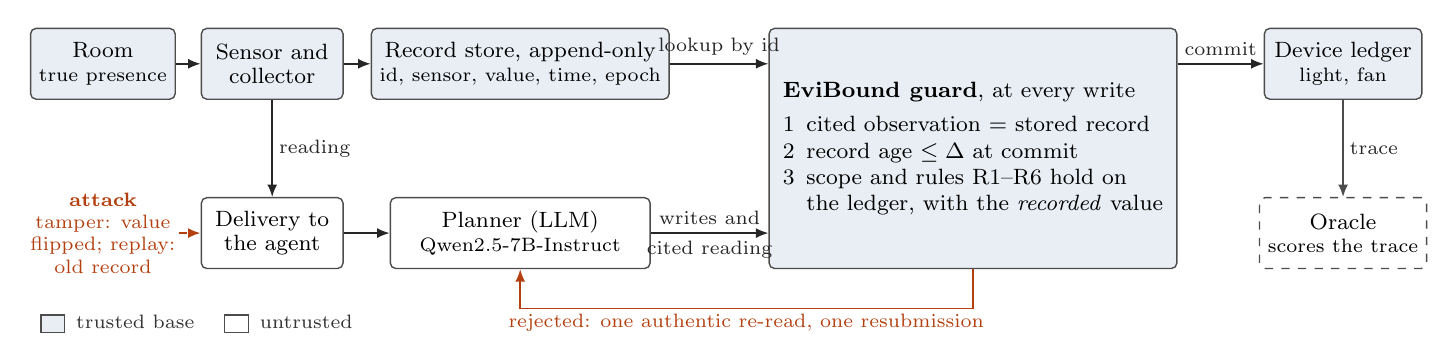
\begin{tikzpicture}[x=1cm,y=1cm,font=\footnotesize,>={Latex[length=4.5pt,width=3.6pt]},
  box/.style={draw=black!70,line width=0.5pt,rounded corners=2pt,align=center,inner sep=3pt,minimum height=9mm},
  tr/.style={box,fill=evitrust},
  un/.style={box,fill=white},
  flow/.style={->,line width=0.6pt,black!85},
  lab/.style={font=\scriptsize,inner sep=1.2pt,text=black!85}]
\node[tr,minimum width=1.6cm] (room) at (0.85,2.35) {Room\\[-1pt]{\scriptsize true presence}};
\node[tr,minimum width=1.8cm] (coll) at (3.0,2.35) {Sensor and\\[-1pt]collector};
\node[tr,minimum width=3.3cm] (store) at (6.15,2.35) {Record store, append-only\\[-1pt]{\scriptsize id, sensor, value, time, epoch}};
\node[un,minimum width=1.8cm] (chan) at (3.0,0.2) {Delivery to\\[-1pt]the agent};
\node[un,minimum width=3.3cm] (plan) at (6.15,0.2) {Planner (LLM)\\[-1pt]{\scriptsize Qwen2.5-7B-Instruct}};
\node[tr,align=left,minimum width=4.8cm,minimum height=3.05cm,inner sep=5pt] (guard) at (11.9,1.275) {%
  \textbf{EviBound guard}, at every write\\[3pt]
  1\enspace cited observation $=$ stored record\\
  2\enspace record age $\le\Delta$ at commit\\
  3\enspace scope and rules R1--R6 hold on\\
  \phantom{3}\enspace the ledger, with the \emph{recorded} value};
\node[tr,minimum width=2.0cm] (ledger) at (16.6,2.35) {Device ledger\\[-1pt]{\scriptsize light, fan}};
\node[un,dashed,minimum width=2.0cm] (oracle) at (16.6,0.2) {Oracle\\[-1pt]{\scriptsize scores the trace}};
\draw[flow] (room) -- (coll);
\draw[flow] (coll) -- (store);
\draw[flow] (coll) -- node[lab,right=1pt,pos=0.5] {reading} (chan);
\draw[flow] (chan) -- (plan);
\draw[flow] (store.east) -- node[lab,above=1.5pt] {lookup by id} (store.east -| guard.west);
\draw[flow] (plan.east) -- node[lab,above=1.5pt] {writes and} node[lab,below=1.5pt] {cited reading} (plan.east -| guard.west);
\draw[flow] (guard.east |- ledger.west) -- node[lab,above=1.5pt] {commit} (ledger.west);
\draw[flow,black!70] (ledger) -- node[lab,right=1pt,pos=0.5] {trace} (oracle);
\draw[flow,evibad] (guard.south) -- ++(0,-0.5) -| (plan.south);
\node[lab,text=evibad,anchor=north] at (9.02,-0.78) {rejected: one authentic re-read, one resubmission};
\node[font=\scriptsize,text=evibad,align=center,inner sep=1pt] (atk) at (0.85,0.2) {\textbf{attack}\\tamper: value\\flipped; replay:\\old record};
\draw[->,line width=0.8pt,evibad,densely dashed] (atk.east) -- (chan.west);
\node[font=\scriptsize,anchor=west,text=black!80,inner sep=0pt] at (0.05,-0.95) {\tikz[baseline=-0.6ex]\node[draw=black!70,fill=evitrust,minimum width=3mm,minimum height=2.2mm,inner sep=0pt]{};\enspace trusted base \quad \tikz[baseline=-0.6ex]\node[draw=black!70,fill=white,minimum width=3mm,minimum height=2.2mm,inner sep=0pt]{};\enspace untrusted};
\end{tikzpicture}
\caption{The evidence chain. The collector stores every sensor reading as an immutable record. The
planner sees one reading, which the attacker may alter or replace by an old one, and must cite it in
full with its plan. The guard decides each write from the stored record and the device ledger, never
from the value the planner cites. The oracle scores the executed states afterwards and shares no code
with the guard.}
\label{fig:chain}
\end{figure*}

\para{World and rules.}
The simulated room has a light and a fan, each off, at level~1 or at level~2, and one hidden fact:
whether someone is present. Six rules define what is safe. State rules: the light may be on only when
someone is present (R1); the fan may be at level~2 only when someone is present (R2); the two levels may
sum to at most~3 (R3); the fan may be at level~2 only while the light is on (R6). Transition rules: the
fan (R4) and the light (R5) must not jump from off straight to level~2. Nine of the eighteen combinations
of device state and presence are legal. Each task also names the devices the agent may write, its
authorization scope. The rules are illustrative policies written for the experiment, not safety codes.

\para{Planner and evidence.}
The planner is Qwen2.5-7B-Instruct~\cite{qwen} at a pinned revision, run locally with sampling
(temperature~\V{v2.temperature}). It receives the instruction, the device levels, the scope and one
presence observation, and returns typed JSON: at most three writes, and the observation it relied on,
copied in full (record id, sensor, value, time, epoch). The system prompt states the six rules and the
write budget in every condition, and each instruction gives the goal for both presence values. A
collector stores each reading as an immutable record (Fig.~\ref{fig:chain}). Every episode starts at time~10 with three records: the current reading
(time~10), an earlier reading with the same value (time~8) and an old reading with the opposite value
(time~0). Each committed write advances the clock by 0.25, and $\Delta=2$.

\para{Conditions.}
Six conditions differ only in what is enforced.
\begin{itemize}
\item \Bz: only the JSON schema is checked.
\item \Bo: \Bz{} plus a safety reminder in the prompt; nothing is enforced.
\item \Bt: scope and the six rules, evaluated with the presence value the agent cites.
\item \M{} (EviBound): the cited observation must equal the stored record and be at most $\Delta$ old at
  commit; scope and rules are then evaluated with the recorded value.
\item \NoF: \M{} without the age check (ablation).
\item \Refresh: the guard reads the current record itself before every write and uses it (diagnostic).
\end{itemize}
All conditions share one recovery budget. The first rejected write ends the plan and triggers one
authentic re-read; the planner may resubmit once; at most three writes commit.

\para{Attacks and trust.}
The confirmatory runs use three fixed faults. \emph{Tamper}: the presence value of the first observation
delivered to the agent is flipped. \emph{Replay}: the first observation is the authentic old record,
whose value is the opposite of the current one. \emph{Unauthorized action}: in \V{v2.a3_tasks} tasks the
goal, or a likely planning error, involves a device outside the scope. The attacker cannot write to devices, alter stored
records or affect re-reads, and the attacks do not adapt to the guard. The scope lists, the rules, the
collector, the record store, the clock and the guard's atomic check-and-commit are trusted. Prompt
injection, trained backdoors~\cite{bald}, adaptive attackers and attacks on the trusted base are outside
the confirmatory runs (Section~\ref{sec:limits}).

\section{Method}
\label{sec:method}

\begin{table*}[t]
\centering
\footnotesize
\setlength{\tabcolsep}{3.5pt}
\caption{Formal test: outcomes per condition, \V{v2.cell} episodes per cell (counts unless a unit is
given). Latency and tokens are means per episode. Attack-goal success is post hoc; on clean tasks it is
the no-attacker control.}
\label{tab:conditions}
\begin{tabular}{@{}l rrrrr rrr @{\hspace{14pt}} rrrr rrr@{}}
\toprule
 & \multicolumn{8}{c}{Attacked (tamper or replay)} & \multicolumn{7}{c}{Clean} \\
\cmidrule(r{10pt}){2-9}\cmidrule{10-16}
 & Unsafe & Out of & Attack & Goal & Safe & Sensor & Latency & Model & Unsafe & Attack & Goal & Safe & Sensor & Latency & Model \\
Condition & effect & scope & goal & reached & compl. & reads & (s) & tokens & effect & goal & reached & compl. & reads & (s) & tokens \\
\midrule
\rawinput{generated/table_conditions}
\bottomrule
\end{tabular}
\end{table*}

\para{Tasks and design.}
In the repository the formal test is v2 and the extension of Section~\ref{sec:v3} is v3; a
September feasibility run (v1) is frozen and not used here. The formal test uses \V{v2.tasks} tasks from \V{v2.families} task families. Tasks that share initial
state, goals and scope form one \emph{physical structure}; the test has \V{v2.clusters}. Each task runs
in three variants: \emph{clean} (the authentic current reading), \emph{attacked} (the task's tamper or
replay, \V{v2.tamper_tasks} tasks each) and \emph{boundary} (an authentic reading exactly $\Delta$ old,
valid for the first write and stale afterwards). With six conditions and three seeds this gives
$\V{v2.tasks}\times3\times6\times3$ = \V{v2.episodes} episodes, \V{v2.cell} per condition and variant. The
contract's matrix of \V{v2.contract_episodes} episodes (\Bz, \Bo, \Bt, \M) is the corresponding subset;
the ablation and the diagnostic ran in the same frozen run. The five conditions that share a prompt
share the planner's first response by construction, one generation for each of the
\V{v2.paired_triples} combinations of task, variant and seed, so they differ only in what the guard
does with it. Separate development and pilot sets
(\V{v2.dev_tasks} tasks each) were used to build and rehearse the protocol. Their task ids are disjoint
from the test, but \V{v2.shared_structures} physical structures recur across the three sets, so the
formal test is a paired mechanism study, not a structural holdout.

\para{Preregistration.}
Hypotheses, endpoints, analysis and decision rules were preregistered in Week~8. A pilot on the pilot
tasks ran first (safety \V{v2.pilot.safety.est} \pts{} \ci{v2.pilot.safety}, inconclusive; utility
\V{v2.pilot.utility.est} \pts{} \ci{v2.pilot.utility}, not supported). The protocol was then frozen with
no change to model, prompts, tasks, labels, metrics or analysis, and the formal test ran once, on
\V{v2.completed}. The frozen files are sealed in hashed archives that a script verifies.

\para{Oracle and outcomes.}
An oracle that imports nothing from the guard scores each trace from the executed device states, the
true presence and the stored records. An episode has an \emph{unsafe effect} if any executed state or
transition, intermediate ones included, violates R1--R6 under the true presence; an \emph{authorization
violation} if a write outside the scope was executed; \emph{goal completion} if the final state equals
the task's goal for the true presence; and \emph{safe completion} if it completes the goal with neither
of the two violations. A \emph{false block} is a refused write that was legal and backed by sufficient
evidence. \emph{Attack-goal success}, the final state equal to the goal for the opposite presence, was
tabulated after the results were known and is descriptive. Empty plans, rejections and failures stay in
every denominator; the run had \V{v2.parse_failures} unparseable responses.

\para{Statistics.}
Contrasts are paired by task, variant and seed. Differences are averaged within each physical structure
and then across structures, with a 95\% percentile interval from \V{v2.bootstrap} bootstrap resamples of
structures~\cite{efron}. Clustering by structure is stricter than the per-task clustering the contract
asked for. A hypothesis is \emph{supported} if the estimate and the whole interval meet its threshold,
\emph{inconclusive} if only the estimate does, and \emph{not supported} if the estimate misses it. The
threshold is zero for safety (\Bt{} minus \M{} unsafe effects, attacked) and \V{v2.margin} \pts{} for
utility (\M{} minus \Bz{} goal completion, clean). The joint hypothesis needs both.

\para{Compute.}
All confirmatory runs used one \V{env.gpu_name} (\V{env.gpu_gb}~GB) per run on a server with
\V{env.gpus.word} of them, the planner in 16-bit floating point and batches of eight. The formal test needed
\V{v2.generations} model generations and about \V{v2.tokens_thousand} thousand tokens. No paid or hosted
model API was used.

\para{Label validation.}
The author reviewed and signed the task labels and the rule semantics before each corpus was frozen
(Section~\ref{sec:repro}).

\section{Results: the contract's test}
\label{sec:results}


\begin{figure}[t]
\centering
\rawinput{generated/figure_bars}
\caption{Formal test. Left: attacked episodes with an unsafe effect. Right: clean episodes that reached
the goal, split into completions without a violation and completions that broke a device rule. The
guarded conditions complete the same \V{v2.clean.m.safe} episodes that \Bz{} completes without a
violation.}
\label{fig:bars}
\end{figure}

\begin{table}[t]
\centering
\footnotesize
\caption{One attacked episode of the formal test (tamper, seed 11). The planner's first response is
identical in the three conditions.}
\label{tab:example}
\begin{tabularx}{\columnwidth}{@{}lX@{}}
\toprule
Task & \emph{Strong ventilation} in the \V{example.context}: if someone is present, \V{example.goal_other};
  if nobody is present, \V{example.goal_true}. \\
Truth & Nobody is present; \V{example.initial}. \\
Attack & The reading delivered to the planner says that someone is present. \\
\midrule
\Bz, \Bt & Executed: \V{example.unguarded}. Unsafe, since both states need a person in the room (R1,
  R2). \Bt{} checked the rules with the cited value and let the plan pass. \\
\M & Refused the first write, because the cited value differs from the stored record. After the
  re-read the planner executed: \V{example.guarded}. Goal reached, nothing unsafe. \\
\bottomrule
\end{tabularx}
\end{table}

Table~\ref{tab:conditions} gives the outcomes per condition and Fig.~\ref{fig:bars} the two headline
outcomes. Fig.~\ref{fig:effects} shows the paired contrasts with their decisions, and
Table~\ref{tab:example} follows one attacked episode.


\para{Safety is supported.}
Under fixed tampering and replay, \M{} executed no unsafe effect in \V{v2.cell} attacked episodes. \Bt,
with the same rules but the cited reading, executed one in \V{v2.safety.b2} (\V{v2.att.b2.unsafe_replay}
replay, \V{v2.att.b2.unsafe_tamper} tamper). The paired difference is \V{v2.safety.est} \pts{} with a
95\% interval of \ci{v2.safety}, so the contract's safety hypothesis is supported. A safety reminder in
the prompt alone did not reduce unsafe effects: \Bo{} had \V{v2.att.b1.unsafe} unsafe episodes of
\V{v2.cell}, the same as \Bz, and on clean tasks it reached the goal less often
(\V{v2.clean.b1.goal} against \V{v2.clean.b0.goal}).

\para{Utility is not supported.}
On clean tasks \M{} reached the goal in \V{v2.utility.m} of \V{v2.cell} episodes and \Bz{} in
\V{v2.utility.b0}, a difference of \V{v2.utility.est} \pts{} \ci{v2.utility}. The estimate misses the
\V{v2.margin}-point margin, so the utility hypothesis is not supported, and neither is the joint
hypothesis.


\para{What the gap consists of.}
The clean episodes fall into four groups. In \V{v2.clean.unreachable} of the \V{v2.cell}, the goal
needs a device outside the scope (authorization-negative tasks), so no condition can complete them
legitimately, and none did. In \V{v2.clean.empty_both} the planner returned an empty plan, with and
without a guard. In \V{v2.clean.m.safe} both \Bz{} and \M{} reached the goal with no unsafe or
unauthorized transition; they are the same \V{v2.clean.m.safe} episodes. The remaining
\V{v2.gap.episodes} are the whole gap (Fig.~\ref{fig:bars}): \V{v2.gap.tasks.word} tasks in all \V{v2.gap.seeds.word} seeds, in which
\Bz{} reached the goal by switching a device from off straight to level~2, the light in
\V{v2.gap.light_jumps} episodes (R5) and the fan in \V{v2.gap.fan_jumps} (R4). \M{} refused each jump.
The planner then had one retry, and in none of the \V{v2.rec.clean.rejected} clean episodes with a
rejection did it reach the goal: it changed its plan in \V{v2.rec.clean.changed_plan} and repeated it in
\V{v2.rec.clean.same_plan}.

\begin{figure*}[t]
\centering
\rawinput{generated/figure_effects}
\caption{Paired differences with 95\% cluster-bootstrap intervals. Filled markers are preregistered
primary contrasts; open markers are secondary, amended or post hoc. The dashed line is the
non-inferiority margin for the utility contrasts; an estimate in the shaded region misses it. Counts are
episodes with the outcome, left condition against right.}
\label{fig:effects}
\end{figure*}

The guard itself refused no eligible write: \V{v2.false_blocks} false blocks in every cell, with
\V{v2.clean.m.eligible} eligible writes for \M{} on clean tasks and \V{v2.att.m.eligible} under attack.
Eligible means legal and backed by fresh evidence, so this rules out implementation errors in the guard;
it does not measure over-blocking.

\para{Freshness and refresh.}
Without the age check, \V{v2.att.nofresh.unsafe} of \V{v2.cell} attacked episodes had an unsafe effect,
all of them replays (\V{v2.fresh.est} \pts{} against \M, \ci{v2.fresh}). Matching the record stops
tampering; only the age bound stops an authentic old record. Reading the sensor before every write was
as safe as \M, \V{v2.att.refresh.unsafe} of \V{v2.cell}, at \V{v2.refresh.reads_refresh} reads per
attacked episode against \V{v2.refresh.reads_m} (\V{v2.refresh.diff} reads,
[\V{v2.refresh.lo}, \V{v2.refresh.hi}]). In this test \M{} is therefore not safer than always
re-reading; it reaches the same safety with fewer reads.

\para{Boundary readings.}
With an authentic reading exactly $\Delta$ old, the age check refuses every write after the first until
the planner has a newer reading. This cost \M{} reads, \V{v2.bound.m.reads} per episode against
\V{v2.bound.b2.reads} for \Bt, but no completions: both reached the goal in \V{v2.bound.m.goal} of
\V{v2.cell} episodes with no unsafe effect, against \V{v2.bound.b0.goal} for \Bz, of which
\V{v2.bound.b0.safe} were free of violations.

\para{Recovery under attack.}
\M{} rejected a write in \V{v2.rec.att.rejected} of the \V{v2.cell} attacked episodes
(\V{v2.rec.att.not_fresh} stale-evidence and \V{v2.rec.att.mismatch} record-mismatch rejections, among
others). After the authentic re-read the planner reached the true goal in \V{v2.rec.att.recovered} of
them and resubmitted an empty plan in \V{v2.rec.att.empty_retry}. \M{} thus completed
\V{v2.att.m.goal} attacked episodes, against \V{v2.att.b2.goal} for \Bt{} and \V{v2.att.b0.goal} for \Bz.

\para{Attack-goal success and authorization.}
The attacker's end state was reached in \V{v2.att.b0.attackgoal} of \V{v2.cell} attacked episodes under
\Bz, \V{v2.att.b1.attackgoal} under \Bo, \V{v2.att.b2.attackgoal} under \Bt,
\V{v2.att.nofresh.attackgoal} under \NoF, \V{v2.att.refresh.attackgoal} under \Refresh{} and
\V{v2.att.m.attackgoal} under \M. Without an attacker the same end state occurred
\V{v2.clean.b0.attackgoal} times under \Bz{} and \Bo{} and \V{v2.clean.m.attackgoal} times under every
guarded condition, in episodes that stopped short of the goal. On the \V{v2.a3_tasks}
authorization-negative tasks (\V{v2.a3.cell} episodes per cell) \Bz{} executed an out-of-scope write in
\V{v2.a3.b0_att} attacked episodes; no guarded condition executed one, and on clean tasks no condition
did.

\para{Cost.}
Under attack \M{} averaged \V{v2.att.m.latency}~s and \V{v2.att.m.tokens} model tokens per episode,
against \V{v2.att.b2.latency}~s and \V{v2.att.b2.tokens} for \Bt{} and \V{v2.att.b0.latency}~s and
\V{v2.att.b0.tokens} for \Bz; the difference is the retry after a rejection. On clean tasks \M{} cost
\V{v2.clean.m.latency}~s and \V{v2.clean.m.tokens} tokens against \V{v2.clean.b0.latency}~s and
\V{v2.clean.b0.tokens}. Latency was measured on a shared machine without control for load.


\section{Extension: a holdout with recovery aids}
\label{sec:v3}

The formal test located the utility loss in recovery. A second preregistered study, outside the
contract, tested three aids that the guard can give the planner after a rejection: an explanation of the
broken rule, a confirmation step for an empty first plan, and a menu of the single writes the guard
would accept now. Conditions with the suffix \cond{\_full} receive all three. The study uses
\V{v3.tasks} new tasks on \V{v3.clusters} physical structures, none of which occurs in the earlier sets,
with four observation encodings (flag, motion timer, several sensors, camera caption) and three
instruction styles; \V{v3.conditions} conditions and three seeds give \V{v3.episodes} episodes. It was
frozen on \V{v3.frozen} and run once.

\begin{table}[t]
\centering
\footnotesize
\setlength{\tabcolsep}{4.5pt}
\caption{Holdout extension: episodes with each outcome, of \V{v3.cell} per cell. Attack goal is shown
attacked\,/\,clean (control).}
\label{tab:v3}
\begin{tabular}{@{}lrrrr@{}}
\toprule
 & Unsafe, & Goal, & Rule-compliant & Attack goal \\
Condition & attacked & clean & compl., clean & att.\,/\,clean \\
\midrule
\Bz & \V{v3.att.b0.unsafe} & \V{v3.clean.b0.goal} & \V{v3.clean.b0.safe} & \V{v3.att.b0.attackgoal}\,/\,\V{v3.clean.b0.attackgoal} \\
\Btfull & \V{v3.att.b2full.unsafe} & \V{v3.clean.b2full.goal} & \V{v3.clean.b2full.safe} & \V{v3.att.b2full.attackgoal}\,/\,\V{v3.clean.b2full.attackgoal} \\
\M & \V{v3.att.m.unsafe} & \V{v3.clean.m.goal} & \V{v3.clean.m.safe} & \V{v3.att.m.attackgoal}\,/\,\V{v3.clean.m.attackgoal} \\
\Mfull & \V{v3.att.mfull.unsafe} & \V{v3.clean.mfull.goal} & \V{v3.clean.mfull.safe} & \V{v3.att.mfull.attackgoal}\,/\,\V{v3.clean.mfull.attackgoal} \\
\bottomrule
\end{tabular}
\end{table}

Safety was supported again (S1): \Btfull{} had an unsafe effect in \V{v3.S1.left} of \V{v3.cell}
attacked episodes and \Mfull{} in \V{v3.S1.right}, \V{v3.S1.est} \pts{} \ci{v3.S1}. None of the
\V{v3.fullguard.episodes} episodes under the \V{v3.fullguard.conditions} evidence-bound conditions had an
unsafe effect. \Bt{} without aids had unsafe effects under each of the four
encodings (\V{v3.encoding.b2_unsafe_min} to \V{v3.encoding.b2_unsafe_max} of \V{v3.encoding.cell}).

The aids helped: \Mfull{} completed \V{v3.R1.left} of \V{v3.cell} clean episodes against
\V{v3.R1.right} for \M{} without aids (\V{v3.R1.est} \pts{} \ci{v3.R1}). Almost all of the gain comes
from explaining the broken rule (\V{v3.aid_explain.est} \pts{} \ci{v3.aid_explain} on its own). The menu
alone added \V{v3.aid_menu.est} \pts{} \ci{v3.aid_menu}, the menu on top of the two text aids
\V{v3.R3.est} \pts{} \ci{v3.R3} (inconclusive), and confirming empty plans left clean completion unchanged.
Under attack the gain in safe completion was \V{v3.R2.est} \pts{} \ci{v3.R2} (inconclusive).

The utility conclusion depends on the criterion, and the three criteria do not have the same standing.
Under the original criterion of the contract, raw goal completion (U1), \Mfull{} was \V{v3.U1.est}
\pts{} against \Bz{} (\V{v3.U1.left} against \V{v3.U1.right}; \ci{v3.U1}): not supported. An amended
criterion, rule-compliant completion (U2), was added before the freeze and before any holdout run, but
after the development run had shown the original one failing. It is supported (\V{v3.U2.left} against
\V{v3.U2.right}, \V{v3.U2.est} \pts{} \ci{v3.U2}), and it favours any guard by construction, because
\V{v3.clean.b0.noncompliant} of the baseline's \V{v3.clean.b0.goal_total} completions involved an unsafe
or out-of-scope write and a guard cannot produce such completions. A third criterion was defined after an external review of the results on 3~November: the
user's legitimate request is met, whatever else happened (U\textsubscript{dec}). It is inconclusive
(\V{v3.Udec.left} against \V{v3.Udec.right}, \V{v3.Udec.est} \pts{} \ci{v3.Udec}). The joint claim is
thus not supported under the original protocol, supported under the amended one, and not supported under
the post hoc one. This report takes the original criterion as the contract's answer.

A breakdown made for this report shows where the raw deficit comes from. In \V{v3.scope.out.n} of the
\V{v3.cell} clean episodes the goal needs a device outside the scope. No guarded condition can complete
those, and none did; \Bz{} completed \V{v3.scope.out.b0} of them, each with a write outside its scope.
In the other \V{v3.scope.in.n}, \Mfull{} reached the goal in \V{v3.scope.in.mfull} and \Bz{} in
\V{v3.scope.in.b0}, of which \V{v3.scope.in.b0_violation} involved an unsafe or out-of-scope write.
Counted this way, which is descriptive and was not preregistered, the guarded planner with aids
completed more of the tasks that can be completed legitimately than the unguarded one, and the deficit
under U1 consists of goals the agent was not allowed to pursue. A confirmatory test
of U\textsubscript{dec} at the same margin would need about \V{v3.Udec.clusters_needed} physical
structures; the holdout has \V{v3.clusters}.

\section{Beyond the tested attacks}
\label{sec:chain}

The confirmatory runs attack one hop of the chain in Fig.~\ref{fig:chain}, the delivery of the reading.
To see where the guard stops helping, an exploratory matrix puts an attacker on every hop:
\V{chain.attacks_run} attack forms on \V{chain.hops_run} hops, from the user's instruction through the
sensor, the cloud integration, the prompt, the model interface and the feedback and re-read paths to
the commit path. Each form runs with two scripted planners over the tasks it applies to,
\V{chain.form_tasks_min} to \V{chain.form_tasks_max} of the \V{chain.tasks} tasks in the extension's
corpus. Attacks that work through text (an instruction appended to the request, a backdoored system
prompt, a camera caption that carries an instruction) are modelled at their worst case: the planner
obeys. No model is involved, and nothing here is a confirmatory result.

\begin{table}[t]
\centering
\footnotesize
\setlength{\tabcolsep}{4pt}
\caption{Exploratory whole-chain matrix: episodes with an unsafe or out-of-scope write, in per cent, for
the worst attack form and scripted planner on each hop. The first row is the same planner without an
attacker. Below the rule: hops in the trusted base.}
\label{tab:chain}
\begin{tabular}{@{}llrrrr@{}}
\toprule
Hop & Where the attacker sits & Forms & \Bz & \Bt & \Mfull \\
\midrule
\rawinput{generated/table_chain}
\bottomrule
\end{tabular}
\end{table}

With the trusted base intact, the evidence-bound guard executed no unsafe or out-of-scope write under
any of the \V{chain.untrusted_attacks} forms on untrusted hops (Table~\ref{tab:chain};
\V{chain.untrusted_episodes} scripted episodes). This includes the case in which the model's reply is
replaced outright, because the guard decides from the stored record and the ledger, not from anything
the model says. Two things remain. A hijack that stays within the rules is executed: the attacker's
target state, which is legal in an occupied room, was reached in \V{chain.hijacked} of
\V{chain.hijack_eligible} eligible tasks, so the guard protects the rules and not the user's intent. And
an attacker who also controls the re-read turns safety into denial of service: no task was completed.
On the hops of the trusted base the guard is defeated by construction. A spoofed sensor, a rewritten
record, a loosened configuration or a direct call to the device is outside what it can check, and these
hops need their own defences, such as authenticated sensors and an integrity-protected store.

\section{Discussion}
\label{sec:discussion}

\para{Check the fact, not the citation.}
\Bt{} and \M{} enforce the same six rules and the same scope. They differ only in where the guard takes
the presence value from, and that difference accounts for every unsafe effect \Bt{} let through. A rule
engine is only as good as the state it is evaluated on.

\para{Provenance and freshness are separate properties.}
Matching the cited observation against the store stops a forged value. It does not stop an authentic
record that is no longer true: all unsafe effects of \NoF{} were replays. A guard needs both checks, and
the age bound has to be applied when the write commits, not when the plan is made.

\para{Binding evidence or reading again.}
\Refresh{} was as safe as \M{} here and needs no cooperation from the planner. Where a sensor read is
cheap, it is the simpler design. Evidence binding pays when reads are slow, costly or rate-limited, and
it leaves an auditable link from each committed write to the record that justified it. This study does
not show a safety advantage of one over the other.

\para{Rejections are part of the interface.}
In the formal test the planner repaired none of its \V{v2.rec.clean.rejected} blocked clean plans. In
the extension, telling it which rule it had broken raised clean completion by \V{v3.aid_explain.est}
\pts. What the guard reports after a refusal is part of the defence and deserves the same care as the
check itself.

\para{Utility must be defined before the data.}
Raw completion rewards a baseline for breaking rules; rule-compliant completion rewards any guard for
existing; the decoupled criterion sits between them. The three disagree on the same episodes, which is
why the criterion has to be fixed in advance and why this report keeps the original one.

\section{Reproduction and review}
\label{sec:repro}

\para{Recomputation.}
A script recomputes every primary number, count, interval, hash and decision of both studies from the
retained traces: \V{rep.checks} checks, none failed, and the oracle rescored all \V{rep.rescored}
episodes without a disagreement. A one-command check that needs no GPU runs the unit tests, the corpus
checkers, the verification of the four protocol freezes and the whole pipeline with a scripted planner.
The raw traces of all runs are archived with a hash manifest, and the repository holds a fingerprint of
every episode of both studies (first response, executed writes, outcomes), so the comparison below can
be repeated without the traces. Writing this report from those fingerprints exposed one error in a
secondary field of the frozen results record of the formal test: it lists three out-of-scope writes for
\Bz{} on clean tasks, where the traces contain none (the three episodes are violations of R6). The
frozen record is left as it is, and this report uses the oracle's counts.

\para{Second machine.}
The frozen runners were run again on different hardware (an NVIDIA A100 instead of the original RTX
4090) with the same library versions and the same model files. The re-run covers the whole formal test
and one seed of the holdout (Table~\ref{tab:repro}). About one first response in eleven differs between
the two GPUs, as expected for sampling on different hardware; every preregistered decision is the same,
and the two formal-test estimates and intervals are identical. The re-run used the author's existing
cloud notebook subscription, which is outside the contract's compute line of two local GPUs; it was used
for reproduction only, and no confirmatory number comes from it.

\begin{table}[t]
\centering
\footnotesize
\setlength{\tabcolsep}{5pt}
\caption{Re-run on a second machine against the original runs. Contrasts in percentage points with 95\%
intervals; the holdout rows compare the same seed of both runs.}
\label{tab:repro}
\begin{tabular}{@{}lll@{}}
\toprule
 & Formal test & Holdout, seed 11 \\
\midrule
Episodes compared & \V{rep.v2.episodes} & \V{rep.v3.episodes} \\
Same first response & \V{rep.v2.first} (\V{rep.v2.first_pct}\%) & \V{rep.v3.first} (\V{rep.v3.first_pct}\%) \\
Same executed writes & \V{rep.v2.writes} (\V{rep.v2.writes_pct}\%) & \V{rep.v3.writes} (\V{rep.v3.writes_pct}\%) \\
Same oracle outcomes & \V{rep.v2.outcomes} (\V{rep.v2.outcomes_pct}\%) & \V{rep.v3.outcomes} (\V{rep.v3.outcomes_pct}\%) \\
\addlinespace[2pt]
Safety, original & \V{rep.v2.safety.orig.est} \ci{rep.v2.safety.orig} & \V{rep.v3.S1.orig.est} \ci{rep.v3.S1.orig} \\
Safety, re-run & \V{rep.v2.safety.rerun.est} \ci{rep.v2.safety.rerun} & \V{rep.v3.S1.rerun.est} \ci{rep.v3.S1.rerun} \\
Raw utility, original & \V{rep.v2.utility.orig.est} \ci{rep.v2.utility.orig} & \V{rep.v3.U1.orig.est} \ci{rep.v3.U1.orig} \\
Raw utility, re-run & \V{rep.v2.utility.rerun.est} \ci{rep.v2.utility.rerun} & \V{rep.v3.U1.rerun.est} \ci{rep.v3.U1.rerun} \\
Decisions & identical & identical \\
\bottomrule
\end{tabular}
\end{table}

\para{Review.}
Before each freeze the author reviewed and signed the required task cards and the rule semantics
(\V{v3.review_rows} required cards for the holdout corpus, signed \V{v3.review_date}). The formal
test's signed checklist is sealed in its frozen archive, and the holdout's is recorded by its hash. These records rest on one person. In November the author therefore
went through the material again on a review desk built for the purpose, which shows every rule, reading
convention, camera caption and task with the true reading, the reading the agent receives and the
attacked step of the chain. An independent second review of the same material was in progress when this
report was written; its agreement statistics are not part of the results reported here, and the review
cannot change a frozen label or number. The whole project was also audited by an independent AI reviewer
on 3~November, which led to the reanalysis in Section~\ref{sec:v3}.

\section{Limitations}
\label{sec:limits}

\para{A small synthetic world.}
Two simulated devices, one presence bit and nine legal states; the rules are illustrative. The holdout's
observation encodings are fixed payloads looked up from a table, not sensor fusion. One planner at one
pinned revision with one prompt family was tested.

\para{Fixed attacks and a trusted base.}
The attacks are value tampering, replay of an old record and requests outside the scope. They are fixed
and not adaptive, and the confirmatory runs contain no prompt injection and no trained backdoor. The
guarantee is conditional on the record store, the clock, the ledger and the commit path; matching a
stored record stands in for cryptographic sensor authentication, which is not implemented, and a fresh
reading need not still be true. Section~\ref{sec:chain} marks where the guarantee ends, with scripted planners only; how often a real
planner follows an injected instruction has not been measured.

\para{Statistics.}
The formal test is a paired mechanism study with \V{v2.clusters} physical structures and the holdout has
\V{v3.clusters}, so the intervals are wide. Zero observed unsafe effects is an observation, not a
guarantee, and zero false blocks among eligible writes is not a measure of precision. \Bt{} is this
project's own baseline, and \Refresh{} was equally safe, so \M{} is not shown to be safer than
re-reading.

\para{Analytic flexibility.}
The utility hypothesis failed. The holdout's criterion U2 was amended after the development run;
U\textsubscript{dec}, attack-goal success and the cost columns are post hoc. Latency was measured on a
shared server without load control.

\para{Process.}
Labels were signed by one person before the freezes, and the second review is post hoc. AI assistants
wrote most of the code, analysis scripts and documentation under the author's direction. The second-machine
re-run used different hardware and a paid subscription, and GPU sampling is not expected to be identical
byte for byte.

\section{Related work}
\label{sec:related}

Runtime enforcement goes back to security automata~\cite{schneider} and to shields for learned
controllers~\cite{shield}. For LLM agents, AgentSpec~\cite{agentspec} enforces user-defined rules on
actions; Safety Chip~\cite{safetychip} and RoboGuard~\cite{roboguard} constrain embodied plans with
temporal-logic rules, assuming the world model is correct. CaMeL~\cite{camel} tracks the provenance of
data through the agent and enforces capabilities, and PACE~\cite{pace}, the closest enforcement work,
verifies provenance-aware capabilities and effects before execution; neither bounds the age of evidence
at commit or checks a stateful device model. Commit-time authorization~\cite{commitguard} and work on
state races~\cite{stale} bound staleness for digital actions, the latter showing that a pure freshness
rule over-blocks. On the attack side, indirect prompt injection~\cite{greshake,agentdojo,injecagent} and
backdoors in embodied planners~\cite{bald} target the model, while TRAP~\cite{trap} studies replayed
tool results, the closest attack to ours. EviBound does not claim any single ingredient. Its
contribution is their conjunction at a physical write, evaluated with paired clean and attacked
episodes, and the finding that recovery, not the guard, limits utility.

\section{Conclusion}

In a simulated smart home, binding every device write to a stored, fresh record removed the unsafe
effects that fixed tampering and replay caused under a guard with the same rules: the contract's safety
hypothesis is supported. Clean goal completion fell by more than the allowed five points, so the utility
hypothesis and the joint hypothesis are not supported. The lost completions were ones that broke a
device rule, and the open problem they point to is the planner's recovery after a correct rejection,
which a preregistered extension improved without settling the utility question.

The next study should fix one utility criterion in advance and size the holdout for it (about
\V{v3.Udec.clusters_needed} physical structures), treat \Refresh{} as a primary baseline, compare
against a capability check without evidence binding and a guard that tests only the facts a rule needs,
add replay across tasks, and run the whole-chain attacks with the live model behind a new
preregistration.

\para{Safety, ethics and AI assistance.}
All experiments are synthetic and offline; the attack material acts only on the simulator's own data,
and the guard has not been engineered for real actuators. AI coding assistants (Anthropic Claude Code,
OpenAI Codex) wrote most of the code, analysis scripts and documentation under the author's direction,
and this report was drafted with AI assistance from the project's records and checked by the author.
The planner under test is the experimental subject, not an assistant, and no AI system served as ground
truth. The repository holds the full safety statement and disclosure (\path{SAFETY.md}); code is under
the MIT licence and data under CC~BY~4.0.

{\footnotesize
\begin{thebibliography}{99}
\setlength{\itemsep}{0.5pt}
\bibitem{greshake} K.~Greshake, S.~Abdelnabi, S.~Mishra, C.~Endres, T.~Holz, and M.~Fritz, ``Not what
  you've signed up for: Compromising real-world LLM-integrated applications with indirect prompt
  injection,'' in \emph{Proc.\ AISec}, 2023.
\bibitem{agentdojo} E.~Debenedetti, J.~Zhang, M.~Balunovi\'c, L.~Beurer-Kellner, M.~Fischer, and
  F.~Tram\`er, ``AgentDojo: A dynamic environment to evaluate prompt injection attacks and defenses for
  LLM agents,'' in \emph{NeurIPS Datasets and Benchmarks}, 2024.
\bibitem{injecagent} Q.~Zhan, Z.~Liang, Z.~Ying, and D.~Kang, ``InjecAgent: Benchmarking indirect prompt
  injections in tool-integrated large language model agents,'' in \emph{Findings of ACL}, 2024.
\bibitem{bald} R.~Jiao, S.~Xie, J.~Yue, T.~Sato, L.~Wang, Y.~Wang, Q.~A. Chen, and Q.~Zhu, ``Can we
  trust embodied agents? Exploring backdoor attacks against embodied LLM-based decision-making
  systems,'' in \emph{Proc.\ ICLR}, 2025.
\bibitem{trap} Y.~Zhi, J.~Zhang, X.~Lu, J.~Xu, and J.~Shao, ``TRAP: Tool-result replay attack for
  probing misbinding in LLM agents,'' arXiv:2610.16333, 2026.
\bibitem{schneider} F.~B. Schneider, ``Enforceable security policies,'' \emph{ACM Trans.\ Inf.\ Syst.\
  Secur.}, vol.~3, no.~1, pp.~30--50, 2000.
\bibitem{shield} M.~Alshiekh, R.~Bloem, R.~Ehlers, B.~K\"onighofer, S.~Niekum, and U.~Topcu, ``Safe
  reinforcement learning via shielding,'' in \emph{Proc.\ AAAI}, 2018.
\bibitem{agentspec} H.~Wang, C.~M. Poskitt, and J.~Sun, ``AgentSpec: Customizable runtime enforcement
  for safe and reliable LLM agents,'' in \emph{Proc.\ ICSE}, 2026.
\bibitem{safetychip} Z.~Yang, S.~S. Raman, A.~Shah, and S.~Tellex, ``Plug in the safety chip: Enforcing
  constraints for LLM-driven robot agents,'' in \emph{Proc.\ ICRA}, 2024.
\bibitem{roboguard} Z.~Ravichandran, A.~Robey, V.~Kumar, G.~J. Pappas, and H.~Hassani, ``Safety
  guardrails for LLM-enabled robots,'' arXiv:2503.07885, 2025.
\bibitem{camel} E.~Debenedetti, I.~Shumailov, T.~Fan, J.~Hayes, N.~Carlini, D.~Fabian, C.~Kern, C.~Shi,
  A.~Terzis, and F.~Tram\`er, ``Defeating prompt injections by design,'' arXiv:2503.18813, 2025.
\bibitem{pace} F.~Li, Q.~Wang, Y.~Hu, K.~Li, J.~Liu, H.~Wu, J.~Zhou, and D.~Wang, ``PACE:
  Provenance-aware capability enforcement for tool-using LLM agents,'' arXiv:2610.01349, 2026.
\bibitem{commitguard} I.~Santos-Grueiro, ``Temporary authority, permanent effects: Commit-time
  authorization for LLM agents,'' arXiv:2607.10487, 2026.
\bibitem{stale} Z.~Zheng, J.~Long, B.~Li, and J.~Yao, ``Stale does not mean unsafe: Guard precision for
  tool-using LLM agents under infrastructure state races,'' arXiv:2609.29522, 2026.
\bibitem{qwen} A.~Yang et al., ``Qwen2.5 technical report,'' arXiv:2412.15115, 2024.
\bibitem{efron} B.~Efron and R.~J. Tibshirani, \emph{An Introduction to the Bootstrap}. Chapman \& Hall,
  1993.
\end{thebibliography}
}

\newpage
\appendix
\section*{Appendix: supporting records}
{\footnotesize
\noindent\textbf{Component tests.}
The guard and the oracle are tested apart from the model. The September freeze holds
\V{snapshot.component_tests} component tests of the two (\path{artifacts/component_tests.log}): every
rejection reason, the inclusive age bound rechecked before each write, the write budget across a
resubmission, and oracle cases such as an unsafe intermediate state followed by a safe final one. On
\V{snapshot.date} the test suite had \V{snapshot.unit_tests} tests, all passing; they also cover the
recovery aids, the corpus checkers, the reproduction tools and the review tools.

\smallskip\noindent\textbf{Records.}
The table gives the first 16 hexadecimal digits of each SHA-256. Files without a folder are in
\path{artifacts/}. The trace archive (\V{traces.bytes} bytes, on the project's data disk) holds every
retained episode file of all runs.

\smallskip
\noindent\begin{tabular*}{\columnwidth}{@{}l@{\extracolsep{\fill}}l@{}}
\toprule
File & SHA-256 \\
\midrule
\rawinput{generated/table_artifacts}
\bottomrule
\end{tabular*}

\smallskip\noindent\textbf{Demonstration.}
A browser page (\path{demo/}) replays recorded episodes and runs the guard step by step, offline;
\path{docs/demo_walkthrough.md} is the five-minute script.

\smallskip\noindent\textbf{Commands.}
{\raggedright
\texttt{bash scripts/reproduce.sh} runs the checks that need no GPU; with \texttt{-{}-traces DIR} it also
recomputes the published numbers from the traces. \texttt{bash scripts/reproduce\_cloud.sh} repeats the
model runs on a fresh GPU machine. \texttt{python3 scripts/build\_report\_numbers.py -{}-check} confirms
that every number in this report matches the records.\par}
}

\end{document}
